\documentclass[output=paper]{LSP/langsci}
\author{Effie Mouka, Ioannis E. Saridakis and Angeliki Fotopoulou}
\title{Racism goes to the movies: A corpus-driven study of cross-linguistic racist discourse annotation and translation analysis}
%\epigram{Change epigram in chapters/01.tex or remove it there}
\abstract{This paper traces register shifts (\citealt[22]{HallidayHasan1976}; \citealt{Hatim1997}) between source-texts (English) and target-texts (Greek and Spanish) in instances of racist discourse in films. It presents preliminary, as yet non-exhaustive, findings and aims to ultimately formulate explanatory hypotheses concerning the emerging norms. Our methodological approach is placed in the framework of Descriptive Translation Studies \citep{Toury2012,Chesterman2008} and in the school of Critical Discourse Analysis \citep{Fairclough1985,Fairclough1992}, relying on Appraisal Theory \citep{MartinWhite2005} to provide and analyse a taxonomy of the racism-related utterances examined.}
\maketitle

\begin{document}

\section{Introduction} \label{sec:2:1}
Technological advances in Corpus Linguistics and tools for processing and compiling linguistic corpora open new ways on how we exploit textual and research material. In a descriptive approach, textual and pragmatic annotation can largely facilitate the systematic lexico-grammatical analysis of linguistic resources (\citealt[29-31]{EneryHardie2012}; \citealt[76-79]{Zanettin2012}). This holds true also for translation corpora, with a particular focus on the descriptive examination of translation strategies and norms \citep[78-96]{Zanettin2012}.

This paper partly presents the first author's\footnote{The second author, I.E. Saridakis is the PhD research director. Dr. A. Fotopoulou also participates in the consultative committee of the project. The authors express their gratitude to V. Giouli, scientific associate at the Institute for Language and Speech Processing (ILSP) for her support in initially developing and implementing the sentiment annotation scheme described in this paper, and in adopting the corpus metadata handling model used in our method.} ongoing PhD research, which aims to examine, from a descriptive viewpoint and by using corpus annotation, the translational norms of the socio-culturally marked discourse of racism, and the shifts observed during the discourse transfer from a source language (EN) into two target languages (EL, ES)\footnote{\citet[120-121]{Batsalia2010} define “shifts” as subsuming all changes that may appear during the translation process, on a semantic, lexical, morphological, syntactic, pragmatic, and/or stylistic level. The “translation shift” hypothesis is a useful and powerful descriptive device, to approach hermeneutically the phenomenon of differentiation of the \textsc{tt} from its \textsc{st}, without stigmatising it.}. This paper focuses on the applied methodology, on the findings collected so far, and discusses problems and impediments observed during corpus analysis.

Racism, as manifested in discourse, is a constantly open issue that merits research \citep{Dijk1993,Reisigl2001} and is clearly on the agenda of (critical) discourse analysis in light of the European social, political and economic backdrop. Realistic films on racism represent discourses emanating from racist stances, while cinema, as a medium widely accessible to the public communicates ideas apart from reflecting society. On the other hand, subtitles are considered to be among the most read translations and text types in countries with a subtitling tradition (\citealt[153]{Gottlieb1997} in \citealt[125]{Pedersen2011}). To this end, the analysis of subtitles in racism-related films, rather than in films with sporadic racist utterances, seems to be better suited to research on the translation of racist-oriented discourse.

\sectref{sec:2:2} of this article outlines the aims and scope of our research, and introduces the basic concepts and theoretical tenets used in this study. First, we introduce the principal discourse-related definitions of racism, together with a discussion of how racist discourse is handled by Critical Discourse Analysis. Subsequently, we provide a brief overview of Appraisal Theory, first developed by \citet{MartinWhite2005}. This theory has been used extensively in sentiment analysis. Finally, we consider the phenomenon of register shifts in subtitles.

\sectref{sec:2:3} presents our corpus-driven methodology and the corpus tools used in our research. \sectref{sec:2:4} and \sectref{sec:2:5} present and exemplify the implementation of our methodology and outline the principal findings with regard to context-bound register shifts in translation.

\section{Research aims and scope} \label{sec:2:2}
The focus of our work is to examine racist discourse from a translation perspective, identifying its structure, its textual deployment, and its elements and traits on the basis of lexicogrammatical evidence and using a classificatory device. In other words, our aim is to examine how racist attitudes can be classified in spoken film discourse, linking this classification to the context of the utterances from which the text chunks have been drawn. This classification and analysis is based on a model adapted from Appraisal Theory \citep{MartinWhite2005}, using postulates derived from Critical Discourse Analysis \citep{Reisigl2001,Dijk2000a,Dijk2000b,Dijk2002}. Finally, by linking the examined \textsc{st} utterances to their translations in two TLs, register shifts can be analysed on the basis of previous research \citep{Hatim1997, Mason2001, Pettit2005, Mubenga2009, Munday2012}.
This study is based on corpus resources and methodologies. We first constructed an ad hoc corpus and annotated it with a purpose-built annotation scheme, then set out to identify register shifts in the translation of racist utterances. This approach is exemplified by the preliminary findings reported in this article.

\subsection{Background. Racism and racist discourse} \label{sec:2:2:1}
The phenomenon of racism is fuzzy and evasive, and the term is often used rather vaguely, even to describe discriminatory phenomena other than those related to the concept of “race”. \textit{Racism} subsumes everyday practices and behaviours, both verbal and non-verbal, stereotyping, discriminatory practices, institutional systemic policies, or even acts of racial segregation and genocides \citep[637-653]{Giddens2009}.

How racism is defined depends, in the final analysis, on the scope of each research: for example, literature lists distinctive definitions such as “institutional” or “systemic” racism, to designate racism that is present in societal structures, such as the educational system or the police; “neo-racism” or “cultural racism” that draws from cultural differences in an attempt to provide explanations for inequalities and the actual position of ethnic minorities, immigrants and refugees in society, as opposed to the “old-style” and merely biologically explained racism that is based on physical characteristics to sustain the inferiority of certain group members; “everyday racism” as a common societal behaviour; or racism as part of the wider phenomenon of “heterophobia”, the fear of the Other, that gives birth to various forms of discrimination (\citealt{Essed1991,Reisigl2001}; \citealt[118]{Memmi2000}). Racism has “the cognitive function of organizing the social representations (attitudes, knowledge) of the group, and thus of indirectly monitor[ing] the group-related social practices, and hence also the text and talk of members” \citep[248]{Dijk1995}.

We share Van Dijk's position that ideologies are systems with both a cognitive and a social dimension, in other words “belief systems” that involve ideas, judgements, values and attitudes shared by members of social groups and targeting other social groups.

\subsection{Racism in Critical Discourse Analysis and Corpus Linguistics} \label{sec:2:2:2}
Racist discourse has been investigated mainly within the framework of Critical Discourse Analysis (\textsc{cda}). It has been shown that racist discourse \textit{about} and \textit{addressed at} minorities and immigrants tends to use the following means: lexicon and especially referential and predicative strategies; syntax, i.e. use of passive instead of active voice; rhetorical devices such as metaphors, metonymies and connotations (\textit{synecdoches}); argument schemata; pragmatic features; recurrent topics concerning differences mainly in terms of habits, culture, language or religion of others, or even representations of others as a threat for “our” jobs, safety and culture; standard arguments and fallacies; and local moves or intensifying and mitigation strategies \citep{Reisigl2001,Dijk2000a,Dijk2000b, Dijk2002}.

In a study developing along lines that are ideationally and hermeneutically analogous to the study reported in this paper, \citet{BakerGabrielatos2008} have effectively used a Corpus Linguistics approach to analyse a large corpus of news articles about refugees, asylum seekers, immigrants and migrants and have shown that such an empirical approach can fruitfully combine CL and \textsc{cda}.\footnote{Research in the field of CADS, or Corpus-Assisted Discourse Studies focuses on the use of corpora and corpus analysis techniques, so as to unveil meaning and style in discourse and to examine particular discourses. For a comprehensive bibliography on CADS compiled by C. Gabrielatos, see: \url{http://goo.gl/WHB2mh}.}

\subsection{Appraisal Theory and Sentiment Analysis} \label{sec:2:2:3}
Appraisal Theory is a model that has evolved within the theoretical framework of Systemic Functional Linguistics. It “is concerned with the interpersonal in language, with the subjective presence of writers/speakers in texts as they adopt stances towards both the material they present and those with whom they communicate [...], with how writers/speakers approve and disapprove, enthuse and abhor, applaud and criticise, and with how they position their readers/listeners to do likewise” \citep[1]{MartinWhite2005}. In addition, appraisal “co-articulates interpersonal meaning”\footnote{According to \citet[112]{Halliday1978}, “the interpersonal component represents the speaker’s meaning potential as an intruder. It is the participatory function of language, language as doing something”. Through the interpersonal component, the speaker places himself in the context of the situation, to express also “his own attitudes and judgements” and thus to seek to “influence the attitudes and behaviours of others” (ibid.). In other words, the interpersonal meaning can be defined as the one deriving from the roles and relationships, e.g. status, intimacy, contact, sharedness between interactants \citep[49]{Eggins1997}. Finally, for \citet[94]{Kress2010}, meaning-making is “both social and external and social and internal [...] Meaning is constantly created in a transformative process of interactions with and in response to the prompts of social others and of the culturally shaped environment; and there is constant 'internal' action, an (inner) response in constant engagement with the world”.} \citep[33]{MartinWhite2005}, reflecting the speakers' social roles and interpersonal positioning, and their inter-subjective negotiation. It is an approach that can be used to explore, describe and explain how language is used to express stances.\footnote{In this context, \textit{stance} is meant to represent “performances through which speakers may align or disalign themselves with and/or ironize stereotypical associations with particular linguistic forms” \citep[4]{Jaffe2009}.}

The Appraisal framework has been widely used in Sentiment Analysis to identify subjective information, emotions and opinions, as manifested in discourse \citep[see e.g.][]{Whitelaw2005,Taboada2004,Asher2009} and to classify the attitude of speakers/writers. More recently, this type of analysis has been applied in translation research \citep[see the work reported in][42-79]{Munday2012}, with the aim to “describe the different components of a reader's attitude, the strength of that attitude (graduation) and the ways that the speaker aligns him/herself with the sources of attitude and with the receiver (engagement)” \citep[2]{Munday2012}.

The three sub-components of Appraisal (theory) are \textit{attitude}, \textit{graduation} and \textit{engagement}. \textit{Attitude} is concerned with affect, judgement and appreciation and has a polarity, i.e., a positive or a negative dimension. \textit{Engagement} deals with the positioning of the speaker towards the evaluation and concerns the rhetorical devices that are used to vary the engagement of speakers with their utterances (\textit{I believe}..., \textit{it is rumoured that}..., \textit{X said}....). \textit{Graduation} concerns grading phenomena and adjusting the degree of evaluations (e.g., in the grading between competent player, good player, brilliant player or contentedly, happily, joyously, ecstatically). Moreover, graduation is applicable also to indicators of engagement. A bare assertion does not have the same intensity as an utterance that is introduced with a modal value, such as \textit{possibly} or \textit{certainly} or presented as a hypothesis (compare the following sentences as to the grade of engagement they represent: \textit{They're all a bunch of fucking freeloaders. Some of them are all right \ul{I guess}}) (\citealt[see][136]{MartinWhite2005} for detailed examples of how graduation applies to attitudinal meanings and engagement values).

\subsection{Subtitling: Analysis of register shifts} \label{sec:2:2:4}
The ultimate aim of this study is to analyse register shifts in subtitled films. Munday suggests that “\textit{major shifts in key attitudinal markers are not likely to occur except perhaps in certain genres} [...] where the TL conventions are strongest” \citep[159-160; our emphasis]{Munday2012} and calls for the inclusion of Appraisal Theory in the study of how the interpersonal meaning is materialised in translation (ibid.). Munday regards evaluative expressions in text as critical points that pose problems for translators/interpreters and which are especially susceptible to translators' interventions: he investigates the way a translator's subjective stance is manifested by shifts in translations and concludes that translation choices indicate “both an ideological and axiological position” \citep[155]{Munday2012}. The translator is a critical reader of the original, and he/she is likely either to reproduce the ideological stance of the source text by complying with its general orientation, oppose it by resisting its ideological postulates, or to both reproduce and rework the source in a more tactical approach that repositions the audience in relation to the writer \citep[157]{Munday2012}. Such stance-taking attitudes on the part of the translator–as–critical–reader depend on the overall evaluative prosody of the text, the value of which “the translator sometimes feels obliged to explicate [...] in the interests of the target audience” (ibid.). On a more theoretical line of thought, \citet[215]{Batsalia2010} relate register to style, and speak of stylistic shifts in translation. These are considered to be changes of the language level(s) (i.e. lexical, semantic, pragmatic or morphosyntactic) that can be mapped to stylistic choices. Such choices derive from the translator's own perception of the potential offered by the system of the TL and of the stylistic habits governing the text genre at hand, in a given language. More in particular, subtitling research can optimally incorporate discourse analysis techniques, so as to depict the mechanism through which racism is reflected on cinematographic discourse.

The interpersonal dimension of discourse has been explored using various models in subtitling research. \citet[78-96]{Hatim1997} and \citet{Mason2001} have drawn attention to translation shifts that relate to the interpersonal dynamics of film characters, pointing out that tenor is the metafunction of discourse, which is frequently sacrificed in subtitles. Their analytical approach is that of interpersonal pragmatics, with a focus on politeness features and face-threatening acts. They compare source and target texts using a qualitative method with examples from French films translated into English. On the other hand, \citet{Pettit2005} analyses subtitled and dubbed French versions of two English films, with the aim to examine whether the registers presented in these films are maintained or discarded in the respective subtitled and dubbed versions, providing a variety of examples of formal and informal registers, including slang and sophisticated language. Finally, \citet{Mubenga2009} proposes a multi-modal pragmatic analysis using an SFL approach, which takes into account three components (visual, functional and cognitive) and three levels of analysis (ideational, interpersonal, textual). While sharing the basic assumptions of the above-mentioned studies, our work focuses on register shifts within a specific type of discourse, i.e. racist discourse. Also, in line with \citet{Munday2012}, it relies on Appraisal theory to classify the translators' stance-taking tendencies. We use corpus linguistic techniques to explore translation shifts, by comparing source and target texts in two language pairs.

This study first makes extensive use of linguistic annotation to analyse translational behaviour and to investigate register shifts that take place in racist discourse; subsequently, it validates the data using large monolingual reference corpora. Based on a thorough examination of concordance lines, it provides an analysis of cross-linguistic patterns and of the collocational strength of the lexemes examined.

The aim of cross-linguistic analysis is thus to observe how and to which extent translators have addressed the categories of attitudes, relying on the annotation of register shifts. Using the GATE annotation system \citep{Cunningham2002}, register shifts were classified as \textit{neutral transfer}, \textit{over-toning}, \textit{under-toning}, and \textit{possible change of register category}. This allowed for the retrieval of bilingual segments containing examples of these shifts.


\section{Corpus methodology} \label{sec:2:3}

\subsection{Corpus description} \label{sec:2:3:1}

For the purpose of the present research we have developed a relatively small-scale translational film corpus consisting of the transcriptions of the dialogues of five films in English and their Greek and Spanish subtitles.\footnote{The corpus forms part of the Metashare initiative launched by ELDA (see: \url{metashare.elda.org}). Details on the linguistic resource (“Multilingual aligned corpus of subtitles annotated for sentiment) can be found at \url{http://goo.gl/o45NK5}.}

The criteria used for the design of the corpus relate to the sociolinguistic situation and communicative functions \citep[49-52]{Saridakis2010} of the target population and can be summarised as follows:

\begin{itemize}
\item all films are feature films, belonging to the drama genre;
\item they were all produced between 1989 and 2006 and the frame of reference of their plot is contemporary;
\item their story revolves around racism and inter-racial relations;
\item their approach to events and the depiction of characters have a realistic perspective;
\item they contain verbally expressed racism in conversations and/or in monologues.
\end{itemize}

The five films of the corpus are:

\begin{itemize}
\item \textit{Do the Right Thing} \citep{Lee1989};
\item \textit{American History X} \citep{Kaye1998};
\item \textit{Monster's Ball} \citep{Forster2001};
\item \textit{Crash} \citep{Haggis2004};
\item \textit{This is England} \citep{Meadows2006}.
\end{itemize}

The total playtime of the corpus films corresponds to approximately 9 hours of audiovisual material, which translates into 51,000 words of transcribed English dialogue and 29,700 and 35,900 words of Greek and Spanish subtitles, respectively.

A wide variety of situations involving racist instances is present in our corpus, including both racist discourse \textit{directed} at ethnically different Others, and racist discourse \textit{about} ethnically different Others \citep[351]{Dijk2004}, which equally concern our investigation. The fact that our data contains a significant amount of conversations in inter-racial environments and everyday situations allows us to examine racist discourse \textit{directed at} Others, and overt racist discursive practices. Such features are not always present in corpora of other genres, e.g. in political and journalistic discourse where racism has been studied more extensively using authentic linguistic data\footnote{E.g., in the researches reported in \citet{BakerGabrielatos2008,Dijk1993}, etc.}. Cinematographic discourse can be considered as closely representing spoken impromptu racist discourse, more specifically in utterances that are \textit{directed straight at} Others. Moreover, the communicative scenario from which our samples have been gathered is perhaps the only one permitting the construction of a parallel corpus for the cross-linguistic study of racist discourse from the perspective of translation, given that collecting samples of spoken language from other scenarios is impracticable.

Greek and Spanish were chosen as target languages because their respective cultures share some common characteristics. During the last decades, both Greece and Spain have progressively seen large irregular immigration flows from non-European states, as both countries are key entry-points to Europe. Based on 2013 statistical data, non-European immigrants in Greece and Spain represented respectively 5.96 percent and 6.45 percent of the total country's population.\footnote{See: Eurostat 2014 data \url{http://goo.gl/hbouLx}} It is noteworthy that, with the exception of Greece and Spain, only Italy experiences comparative immigration flows from non-European countries.\footnote{Cmp. \citet[4]{Vasileva2011}; and \url{http://goo.gl/NnhjYR}} In other words, this phenomenon has had a marked impact on the linguistic behaviour (i.e. interpersonal meaning), and therefore on racist discourse, as delineated in this study. However, although immigration is considered to have triggered racist attitudes across Europe, a social survey on racism and xenophobia has shown that the Greek population has quite stronger negative attitudes towards minorities when compared to the Spanish population\footnote{See: Special Eurobarometer 2007. \textit{Discrimination in the European Union} \url{http://goo.gl/t9e6Gk}}. The phenomenon of immigration has had a marked impact on racist discourse and therefore on interpersonal meaning, as negotiated by linguistic behaviour.

A corpus-based approach facilitates the comparison of source and target segments and can help explore the extent of reflection on different socio-cultural realities and attitudes and the effect on the linguistic choices of subtitlers.

In terms of translation practices, previous work in the EL-ES language pair has \textit{inter alia} shown that Greek subtitlers tend to omit repeated or redundant information to a more significant extent when compared to their Spanish counterparts (Sokoli 2009). In short, similar phenomena are bound to be related to generalised tendencies, and this can assist our effort in explicating the textual findings in our corpus.

\subsubsection{Multimodality}
Films are polysemiotic discourse events \citep{Gottlieb2005}. The explication of the meaning of utterances cannot rely solely on the verbal component, but must also take into account its context: “Any consideration of film text in isolation from the context of the moving image and soundtrack is [...] doomed to failure” \citep[23]{Mason2001}.
The audiovisual text is expressed and completed through four semiotic channels \citep{Zabalbeascoa2008}:

\begin{itemize}
\item audio-verbal (words uttered);
\item audio-nonverbal (all other sounds);
\item visual-verbal (writing);
\item visual-nonverbal (all other visual signs).
\end{itemize}

Hence, there can be no valid analysis of the instances of racist discourse if the filmic message is not considered as a whole. The film provided the communicative context for each utterance and for the stance of each character which, additionally, is not static but can change as the plot unfolds. The actual use of the words and its pragmatic features can be deciphered only in this context. “Every clause [...] is a combination of ideational, interpersonal (identity and relational) and textual meanings [...] People make choices about the design and structure of their clauses which amount to choices about how to signify (and construct) social identities, social relationships, and knowledge and belief” (Fairclough 1992: 76). Even apparently innocent lexical choices can indicate a racist stance, while key lexical items are not necessarily racist: a typical example is probably the use of the word \textit{nigger} as an indicator of \textit{belonging} in an otherwise non-racist dialogue between black people:

\begin{quote}
 “You want to get killed, nigger?”\newline
\noindent (\textit{Crash}, in a scene where a black male attempts an armed robbery against the driver of a luxury car and, to his surprise, the driver who resists, is also a black male).
\end{quote}

In this case, the word itself retains its ideological profile and implications as a re-appropriated word. The connotation of key lexical words cannot be taken for granted \textit{a priori} and out-of-context. This is because “the meaning of sentences, clauses, nouns, nominalisations and adjectives are all possible targets for the expression of ideological content, usually in the form of evaluative concepts. In all cases, however, such a semantic representation of opinions in attitudes or models \textit{needs to be analysed in context}” \citep[260; our emphasis]{Dijk1995}.

Moreover, this corpus, comprised of transcribed (i.e. originally oral) \textsc{st}s and written \textsc{tt}s, can also be characterised as a compilation of inter-semiotic facts \citep{Jakobson2012} that imply an inherent change of the mode of the message. Thus, certain features of the \textsc{st}, such as non-standard dialects or code-switching, are not expected to be present in the \textsc{tt}(s). Such features are not usually (or at least, not automatically) transferred to the TL \citep[78]{Hatim1997}. This change implies also that some prosodic features of the source dialogues are not represented in the written subtitles. This holds true also for other non-verbal features, e.g. for gestures. Such features are elements of a semiotic system (the “para-language”) that interrelates with language \citep[32-42]{Halliday2014} and have been used in our analysis in order to properly contextualise and decode the meaning of the \textsc{st}. However, it would be very difficult, and well outside the scope of this study, to trace whether and up to what point the SL and TL audiences decode them in the same way:

\begin{quote}
“Modes differ in what they offer from culture to culture [...]: the different requirements of different societies and their members and the consequent different shaping. As a semiotic resource, \textit{image} in one culture is therefore not identical to \textit{image} in another. Even across closely related cultures and `languages' (such as English, French, German) differences in the cultural use of, say, \textit{vocal intensity} (appearing as \textit{accent} in words and as \textit{rhythm} in extended speech) or of \textit{pitch variation} (appearing as intonation); differences of pace, of \textit{vocalic quality}, and so on, lead to characteristic variation in meanings made, in signs” \citep[81; emphasis in the original]{Kress2010}.
\end{quote}


\subsection{Corpus tools} \label{sec:2:3:2}

We orthographically transcribed the English dialogues and, using ELAN \citep{Brugman2004}, aligned all utterances to the corresponding translated Greek and Spanish subtitles. ELAN is a tool designed for complex annotations of video and audio resources. It allows the use of multiple layers of annotation, which are attributed to each speaker and are time-aligned. In other words, the transcript is aligned to the Greek and Spanish subtitles available in the DVD distributions of the films, thus making the corpus a \textit{star corpus}, i.e. source texts in one language, and their aligned texts in multiple target languages \citep[see][140-141]{Johansson2003}, \citep[see][260]{Saridakis2010}. As shown in \figref{fig:2:1}, the corpus can be expanded to include more target languages in the future, to allow for further cross-linguistic investigations of the translational phenomena. Each utterance is accompanied by a time marker pointing to the corresponding “time-slot” in the film. ELAN allows also the inclusion of metadata to tag the speakers of individual utterances and exports text in \textsc{tei}-compliant \textsc{xml} format using the \textsc{tei}-Drop application \citep{Schmidt2011}, and thus ensures interoperability with the applications used in subsequent stages of our research. The investigator can access the exact point of each utterance, detect the scene from which each utterance has been extracted and reconstruct the communicative context, so as to properly interpret it.

\begin{figure}
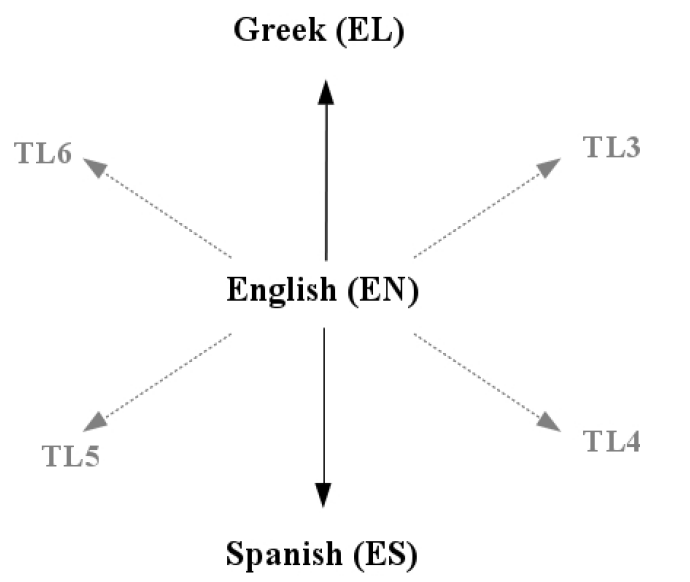
\includegraphics[width=.6\textwidth]{./figures/4-1.png}
\caption{The “star” layout of the study corpus} \label{fig:2:1}
\end{figure}

Concerning the description of the corpus contents, the following metadata has been used (based on the \textsc{tei} guidelines):

\begin{itemize}
\item for files (in the file header section): the audio and video file name/path, the film title, the publication statement (information concerning the distribution of the text);
\item for utterances: information on the speaker (e.g., SPK1 [Danny]), the time-stamp (\textit{anchorsynch}), and the dependent/aligned tiers with the Greek and Spanish translations respectively (\textit{spanGrp} type).
\end{itemize}

An example of an \textsc{xml}-tagged utterance and of its translations into EL and ES, as outputted from ELAN following processing in \textsc{tei}-Drop, is in \figref{fig:2:2}.

\begin{figure}
\caption{Example of an \textsc{xml}-tagged utterance} \label{fig:2:2}
\begin{lstlisting}
<div>
<u who="\# SPK1">
<anchor synch="\# T3497"/>
"We are not enemies, but friends.
<anchor synch="\# T3498"/>
</u>
<spanGrp type="subtitles el">
<span to="\#T 3498" from="\# T3497">"Δεν είμαστε εχθροί, αλλά φίλοι.</span> </spanGrp>
<spanGrp type="subtitles es">
<span to="\#T 3498" from="\# T3497">"No somos enemigos, sino amigos.</span> </spanGrp>
</div>
\end{lstlisting}
\end{figure}


ELAN is used to visualise each utterance in its context and its speaker, as well as its aligned subtitled utterances.

\begin{figure}
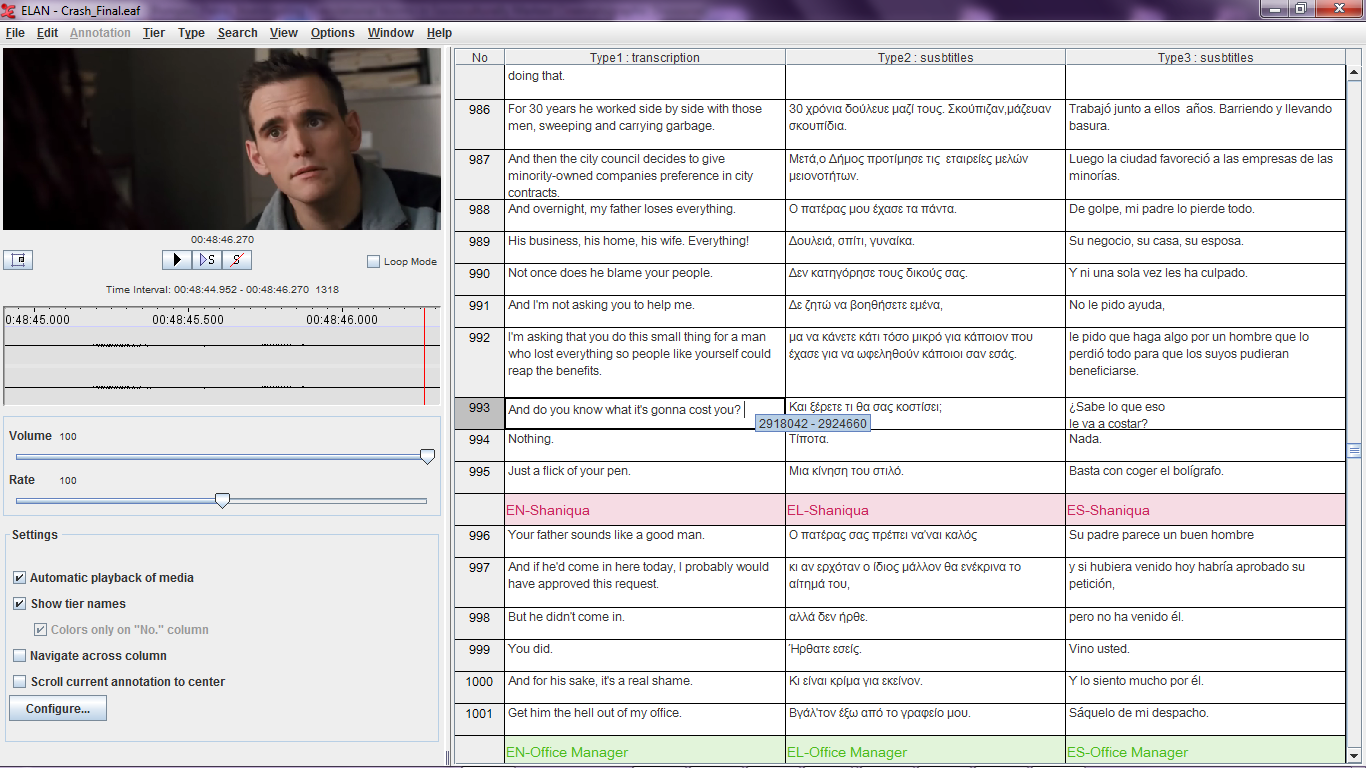
\includegraphics[width=1.0\textwidth]{./figures/4-2.png}
\caption{ELAN interface, in transcription mode}
\end{figure}

To manually annotate the corpus, we have used the GATE platform \citep{Cunningham2002}.\footnote{The annotation methodology and a preliminary annotation scheme (regarding emotions) were first presented in \citet{Mouka2012}. The annotation scheme used in this paper was later finalised and has been reported in \citet{Mouka2014}.} The annotation was performed on the level of text chunks, i.e. of extended units of meaning \citep{Sinclair1996a}. GATE is optimally designed for linguistic annotation. Even though ELAN can also be used for linguistic annotation, it would not be adequate for processing multiple speakers' conversations. ELAN has been primarily developed for psycholinguistic research and each layer of annotation depends on the principal layer attributed to a single speaker. This would be impracticable in the case of our corpus. The change of tool has made impossible the direct access to the audiovisual material and necessitated the simultaneous use of both platforms.

\subsection{Reference corpora} \label{sec:2:3:3}

Although the context of situation provides the main clues on how/why words are used in a specific utterance and what was really meant by it, it cannot be reasonably argued that there is one and only one meaning in each utterance, or a single and precisely determined stance, nor that such meaning or stance can be fully and indisputably perceived and decoded by the analyst. This also applies to our effort to distinguish racist-oriented from neutral discourse elements. What one considers as being blatantly racist or has “labelled” as politically incorrect may be considered “neutral” by others. While well-known racial slurs, such as the lexeme \textit{nigger}, are marked as offensive in all contemporary dictionaries, it can be observed that some of these terms used to be neutral in the past. In order to avoid - as far as possible - being influenced by preconceptions and personal beliefs, especially in view of the cross-linguistic nature of the investigation, the interpretation of how racist markers are used in discourse was based on the evidence provided by reference corpora\footnote{“Reference corpora [...] can be used as benchmarks for special corpora. Whenever we do not want to look at standard language as a whole but at some special phenomenon we happen to be interested in, we usually have to compile a corpus that fits our research focus” \citep[68]{Teubert2007}. In Translation Studies, the use of reference corpora as discourse benchmarks is exemplified, \textit{inter alia}, in \citet[516]{Kenny1998}.}, one for each of the three languages considered.

In the comparative analysis the intuition of the annotator was supplemented with the interpretation of data from the corpora pre-loaded on the SketchEngine platform \citep{Kilgarriff2004}\footnote{\url{www.sketchengine.co.uk}}. These corpora are: enTenTen12 (11+ billion words), GkWaC (124 million words) and esTenTen11 (2.1 billion words), respectively for English, Greek and Spanish.\footnote{For a definition of the TenTen collection of corpora, see \citet{ Jakubicek2013}.} The selected corpora offer texts collected from the Web and, as such, include a variety of text genres and a variety of language uses (both formal and informal). Furthermore, the SketchEngine system allows the visualisation of an extended co-text of concordances. Web corpora also include authentic texts that have not been stylistically filtered and can thus present higher frequencies of informal language, slang and insulting words compared to other general reference corpora (e.g., in the case of Greek, the Corpus of Greek Texts/SEK\footnote{SEK is provided by the University of Athens \url{http://sek.edu.gr}.} and the Hellenic National Corpus/HNC\footnote{HNC is provided by the Institute for Language and Speech Processing (ILSP) \url{http://hnc.ilsp.gr}.}), which usually comprise only authoritative texts or texts that have previously been published in printed form or broadcast and, in that sense, have undergone pre-print editing and perhaps been subjected to cultural and linguistic “filtering” prior to their publication. In most cases, the content of such general reference corpora is “mainstream”/standard texts.\footnote{\citet[65-66]{Teubert2007}, referring to English, define its “standard” form as corresponding to the “private annual reading load of educated middle class citizens” and go on to describe a possible formulation of this definition, in corpus design terms. Such an analogy could also be made for Greek, even though it is not always clear or substantiated how the textual sub-categories would be included in such a corpus.}

\section{Corpus annotation: Analysis and examples} \label{sec:2:4} 
\subsection{Implementing the Appraisal Theory} \label{sec:2:4:1}

This study focuses on the “negative” expressions of racism, i.e., on the discoursal emphasis on negative and/or de-emphasis of positive “things” about \textit{Them}, of which there are many in the corpus. It is beyond our scope to examine the emphasis on positive things and/or the de-emphasis of negative things about \textit{Us}, although these are, more often than not, the other side of the same coin \citep[44]{Dijk2000b}.

For the purposes of our work, we have partially adapted the Appraisal Theory model, by focusing on the classification and “graduation” of attitudes, including the graduation of engagement features, which are labelled “strength” in our schema. Thus, strength is linked to:

\begin{itemize}
\item the valence of an evaluation and its intensification/mitigation; and
\item the intensity of the speaker's engagement with the evaluation, given that our focus is on the degree of the negative attitude expressed by the speaker as a whole.
\end{itemize}

The attitude types used are summarised as follows:
\begin{itemize}
\item \textit{Affect}: emotions and emotional reactions;
\item \textit{Judgement}: evaluation of behaviours;
\item \textit{Appreciation}: evaluation of phenomena, including aesthetics.
\end{itemize}

Our main focus is therefore on exploring the interpersonal nature, the tenor of the discourse and the social relations of the characters of the films, as far as racist stances are manifested in discourse, elements of which are the evaluation of behaviours and situations and the expression of negative emotions and opinions \citep[see][]{Fotopoulou2009}. In this sense, we have categorised and manually annotated “[a]ttitudes [...] divided into three regions of feeling, ‘affect’, ‘appreciation’ and ‘judgement’” \citep[35-43]{MartinWhite2005}. 

For the purposes of our analysis, we annotated every segment of racist attitude of the film characters (appraisers) that express negative evaluations towards a person or a group of another ethnicity/“race”/religion (appraised entity). All candidate instances are interpreted and classified as instantiations of a type of attitude towards “Others”. In this sense, the utterance \textit{Minorities don't give two shits about this country} (American History X), taken semantically, simply informs us about the indifference (affect) of minorities towards \textit{this country}. However, considering how it is used in the given context, we focus on the interlocutor’s intended meaning, which is to implicitly criticise the members of minorities as indifferent free-loaders who just want to exploit the country. Therefore, it is annotated as an implicit judgement.

\subsection{Attitude types and usage perspective} \label{sec:2:4:2}

A systematic classification of racist attitudes requires the clearest possible definition for each category, since the boundaries among attitude types are not always accurate and undoubted. This is not surprising, given that “[i]n a general sense, affect, judgement, and appreciation all encode feeling” \citep[147]{Martin2000}. It cannot be argued that negative judgements or appreciations bear no traces/nuances of affect and that speakers can either express emotions or judge. As a matter of fact, “[a]ffect can perhaps be taken as the basic system […]” (ibid.), as an immanent or emerging characteristic of every attitude. Through this perspective, “[a]s judgement, affect is re-contextualised as an evaluation matrix for behaviour [...] [a]s appreciation, affect is re-contextualised as an evaluation matrix for the products of behaviour (and wonders of nature)” \citep[147]{Martin2000}.

In this sense, we have annotated as instances of \textit{affect} all expressions of emotions, as signs of emotional reactions of the characters related to the specific discourse type. Further, \textit{appreciation} was defined as evaluations, mainly aesthetic, of humans as entities, as evaluations not related to their behaviour but to their characteristics such as colour, ethnicity, religion, physical characteristics and supposed inherent characteristics. Such assessments are negative markers of difference. Finally, \textit{judgement} which “deals with attitudes towards behaviour, which we admire or criticise, praise or condemn” \citep[42]{MartinWhite2005} applies to cases that can be defined as rationalisations of a fact or as reflecting a causal relation between things or facts. On the contrary, in \textit{appreciation}, the speaker's stance is intuitive or dogmatic, i.e. non-refutable in the specific context of situation. In our opinion, this formalisation defines more objectively the classification of attitudes compared to the broader and more inclusive definition offered by \citet[42-45]{MartinWhite2005}.

The basic tri-fold categorisation of attitude as applied in this study is as follows:

\begin{itemize}
\item \textit{Affect}: characterises negative emotions and emotional reactions towards Others, principally instances that are indicative of hate and anger based on or evoked by racial/ethnic/religious differences.
\item \textit{Appreciation}: characterises negative evaluations of Others based on their inherent characteristics, or on characteristics that are presented as such, dogmatically used as sufficient reasons for negative evaluations.
\item \textit{Judgement}: characterises negative evaluations of Others' behaviour, judged as people that act in relation to their racial/ethnic/religious difference.
\end{itemize}

In the paragraphs below, these types are exemplified.

\subsubsection{Affect}

\ea \label{ex:2:1} Your mother, she \emph{hated them niggers} too (\textit{Monster's Ball})
\z
\ea \label{ex:2:2} That means \emph{not welcome} (\textit{American History X}) [utterance addressed to a Jew while the speaker reveals his swastika tattoo]
\z
\ea \label{ex:2:3} Take your fucking pizza piece and \emph{go the fuck back to Africa} (\textit{Do the Right Thing})
\z
\ea \label{ex:2:4} Yeah, \emph{fuck off, you Paki bastards} (\textit{This is England})
\z
\ea \label{ex:2:5} \emph{What the hell are those niggers} doing out there? (\textit{Monster's Ball})
\z

\subsubsection{Appreciation}

\ea \label{ex:2:6} We'll let the \emph{niggers, kikes and spics} grab for their piece of the pie (\textit{American History X})
\z
\ea \label{ex:2:7} A \textit{bunch of people} who \emph{aren't even citizens of this country} [{\dots}] (\textit{American History X})
\z
\ea \label{ex:2:8} She \emph{smells like fish and chips and guacamole} (\textit{American History X})
\z
\ea \label{ex:2:9} Three and a half million of us, who can't find fucking work because \emph{they're taking them all, because it's fucking cheap labour} (\textit{American History X})
\z
\ea \label{ex:2:10} How come \emph{niggers are so stupid}? (\textit{Do the Right Thing})
\z
\ea \label{ex:2:11} Magic, Eddie, Prince, are not \emph{niggers}. I mean, they're not \emph{black}, I mean... (\textit{Do the Right Thing})
\z

\subsubsection{Judgement}


\ea \label{ex:2:12} Look at these little \emph{fucking sewer rats} (\textit{This is England}) [referring to young immigrants playing in a yard]
\z
\ea \label{ex:2:13} \emph{Immigration, AIDS, welfare, those are problems of the black community, the Hispanic community, the Asian community} (\textit{American History X})
\z
\ea \label{ex:2:14} One in every three black males is in some phase of the correctional system. Is that a coincidence or do these people \emph{have like a racial commitment to crime}? (\textit{American History X})
\z
\ea \label{ex:2:15} All right. Well, you know what I can't do? I can't look at you without thinking about the \emph{five or six more qualified white men who didn't get your job} (\textit{Crash})
\z
\ea \label{ex:2:16} He's one of those \emph{proud to be nigger people} (\textit{American History X})
\z

Although “interpersonal epithets” \citep[see][376-377]{Halliday2014}, e.g. evaluative adjectives, are the most obvious evaluative device of language, the lexico-grammatical choices that express attitude are infinite, especially if we consider that evaluative uses of language can be present in discourse both explicitly and implicitly \citep[see][23] {Munday2012}. As shown in the above examples, the lexico-grammatical means to express attitude are vast and not limited to closed semantic or grammatical categories.

In addition, phenomena investigated from another point of view in previous studies are also evident in our data, but are further analysed as instantiations of evaluative attitudes. Referential/nomination strategies and predication strategies, such as racial slurs and metaphors (\textit{sewer rats}) analysed by \citet{Reisigl2001} as a means to categorise membership, are analysed here as evidences of the speaker's stance. Thus, we observe the presence of racial slurs, such as \textit{nigger}, in all three types of attitude:

\begin{itemize}
\item used to express mere anger and hate, as in \REF{ex:2:1} and \REF{ex:2:5},
\item used in appreciations just to refer to Others in a disparaging manner, presenting the fact of belonging to other racial groups and/or having their “inherent” characteristics as being \textit{per se} negative, as in \REF{ex:2:6} and \REF{ex:2:11}, or
\item used in judgements to negatively evaluate a certain person's behaviour, which is presented as related to the fact that he/she is black \REF{ex:2:12}.
\end{itemize}

The interpretation of each instance is based on the context of situation, and is further based on the presence of various markers, either explicitly stated, as in \REF{ex:2:1} where the verb \textit{hate} is used, or using interjections such as \textit{go the fuckback}, \textit{fuck off} and \textit{what the hell} [in \REF{ex:2:3}, \REF{ex:2:4}, and \REF{ex:2:5}].

On the other hand, in \REF{ex:2:6} racial slurs are used instead of “neutral” ethnic denominations as disparaging terms, simply to mark the inferiority of the mentioned groups. The utterance in example \REF{ex:2:11} is a response to the interlocutor's argument that, despite his constant negative attitude towards black people, all his favourite celebrities (Eddie Murphy, Magic Johnson and Prince) are blacks. It is a representative example of how a highly marked racial slur is used as a negative appreciation, to evaluate people as being “nice” or “bad”.

Accordingly, our data includes many convictions and stereotyped visions of Others \REF{ex:2:7} and recurrent topics or \textit{topoi}, as “common-sense reasoning [that is] typical for specific issues” (\citealt{Dijk2000c} in \citealt[299, note 21]{BakerGabrielatos2008}; \citealt[see also][74–76]{Reisigl2001}). Examples are the \textit{topos} of finance \REF{ex:2:9}, the \textit{topos} of threat (\ref{ex:2:13}, \ref{ex:2:14}) and the \textit{topos} of justice or equal opportunities \REF{ex:2:15}. Such visions can be used as appreciations or judgements, i.e. presented as either negative phenomena, as in \REF{ex:2:9}, or as criticism of the behaviour of Others, as in \REF{ex:2:13}, \REF{ex:2:14} and \REF{ex:2:15}.


\subsubsection{Type overlaps}

As mentioned already, it is normal that the boundaries between categories are not always clear-cut: thus, in cases that could belong to more than one category, we have used double annotation: this is both methodologically permissible and of course technically possible. This allows for a subsequent analysis on both levels, e.g. of \textit{affect} and \textit{appreciation}, for the sake of contrastive analysis within the two categories, and hence for further refining the classification/annotation scheme.\newline

\ea \label{ex:2:17} You \emph{gold-teeth, gold-chain-wearing, fried-chicken and biscuit-eating monkey, ape, baboon, big-thigh, fast running, high-jumping, spear chucking, 360-degree basketball-dunking, titsoon, spade, moulignon}!
\z

In this sense, according to our definition of attitudes, the utterance in \REF{ex:2:17} used by an Italian-American in an aggressive manner to express hatred directed to a black person, shows negative affect. At the same time, the long list of epithets enumerated represent appreciations referring to his interlocutor.

\subsection{\textit{Attitude features}} \label{sec:2:4:3}

Attitudes are also analysed in terms of their features.

\subsubsection{Implicit and explicit attitudes} 

As mentioned above, we always categorise attitudes expressed towards persons or groups of other ethnicities/“races”/religions. In many cases, attitudes are not explicitly stated in the text, but evoked, expressed implicitly. Such an interpretation can rely on common knowledge, on the co-text and on the context of the situation.

\begin{quote}
“If by expressing meaning A, language users (also) mean B, such an implication can be reconstructed by recipients only on the basis of inferences from culturally shared knowledge of language meanings (e.g. as represented in the lexicon of the language) or more generally on the basis of shared knowledge, including particular knowledge about the knowledge of the speaker” \citep[168]{Dijk1995}.
\end{quote}

Thus, in example \REF{ex:2:8} above, one should know that \textit{fish and chips and guacamole} refer to the culinary traditions of Latin Americans in order to properly interpret it, whereas in example \REF{ex:2:12} knowledge about the policies of affirmative action against racial discrimination in the USA is crucial in order to interpret the utterance correctly. Moreover, in example \REF{ex:2:12} the term \textit{sewer rat} is used metaphorically to designate useless people that cause problems to society.

\subsubsection{Irony}

Irony is also a case of implicit meaning, a pragmatic phenomenon used to express a meaning contrary or different to the literal one. Once again, its recognition depends on the situational context which indicates something different than the apparent meaning of the utterance, the speaker's tone of voice or the “interpreters' assumptions about the beliefs or values of the text producer”  \citep[123]{Fairclough1992}. For instance, the utterance in example 18 is used to depreciate African-American literature:

\ea \label{ex:2:18} What is it, Black History Month? (\textit{American History X})
\z

\subsubsection{Indirect/Direct attitudes}
Some utterances do not express a racist attitude but are still indicative of the social roles of the participants and can reflect racism as internalised\footnote{\textit{Internalised racism} is defined as the situation in which individuals, groups and cultures that have been subjected to racism and oppression, shift this racism to oppress themselves and others who have experienced racism and discrimination \citep[92]{Lawrence2002}.}. These are cases where speakers comment the racist stance of others and are annotated as indirect references to racist attitudes.\newline

\ea \label{ex:2:19} Man's singing about lynching niggers. “Gonna buy me a rope and lynch me a nigger” (\textit{Crash})
\z
\ea \label{ex:2:20} Your partner's a racist prick (\textit{Crash})
\z

\subsubsection{Polarity}
Polarity refers to the positive or negative dimension of an attitude, distinguishing positive from negative affect, appreciation or judgement. As mentioned already, for the aims of our study we focus on negative instances.

\subsubsection{Strength} 
The strength of each instance is taken into account and an indication of low, medium or high valence is given to each instance. Admittedly, this is the most subjective parameter of our effort, so that in order to decide on the strength of an utterance inter-subjective agreement among the annotators was required in most cases. The collocational behaviour of the lexemes examined was assessed with the help of the English reference corpus.

\subsection{Annotation Scheme Overview} \label{sec:2:4:4}
The attitude classification outlined above and used as annotation scheme in the reported project can be schematised in \figref{fig:2:4}.

\begin{figure}
% 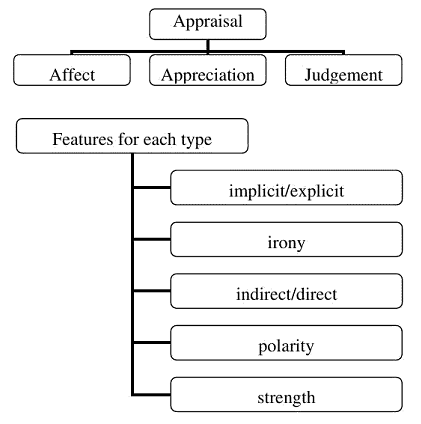
\includegraphics[width=.6\textwidth]{./figures/4-3.png} 
%4-3-Corpus-Annotation-Scheme.tex
\begin{tikzpicture}
[every rectangle node/.style={inner sep=6pt, rounded corners=5, draw}]


\node at (0,0) [rectangle] (appraisal) {Appraisal};
\node [below=5mm of appraisal, rectangle] (appreciation) {Appreciation};
\node [right=20mm of appreciation.east, rectangle] (judgement) {Jugdement};
\node [left=20mm of appreciation.west, rectangle] (affect) {Affect};

\draw [thick] (node cs:name=appraisal, anchor=south) -| (node cs:name=appreciation);
\draw [thick] (node cs:name=affect, anchor=north) |- +(0,.275) -| (node cs:name=judgement);


\node [below right=10mm and 0mm of affect.west, rectangle, text width=40mm, align=center] (features) {Features for each type}; 
\node [below right=4mm and 10mm of features.south, rectangle, text width=40mm, align=center] (implicit) {implicit/explicit};
\node [below=4mm of implicit, rectangle, text width=40mm, align=center] (irony) {irony};
\node [below=4mm of irony, rectangle, text width=40mm, align=center] (indirect) {indirect/direct};
\node [below=4mm of indirect, rectangle, text width=40mm, align=center] (polarity) {polarity};
\node [below=4mm of polarity, rectangle, text width=40mm, align=center] (strength) {strength};

\draw [thick] (node cs:name=features, anchor=south) |- (node cs:name=implicit);
\draw [thick] (node cs:name=features, anchor=south) |- (node cs:name=irony);
\draw [thick] (node cs:name=features, anchor=south) |- (node cs:name=indirect);
\draw [thick] (node cs:name=features, anchor=south) |- (node cs:name=polarity);
\draw [thick] (node cs:name=features, anchor=south) |- (node cs:name=strength);

\end{tikzpicture}
\caption{Corpus annotation scheme} \label{fig:2:4} \todo[inline]{The vector version of this Figure is new. Comments are welcome.}
\end{figure}

\section{Register shifts: Analysis and examples} \label{sec:2:5}

This study investigates how racist/heterophobic discourse is transferred when a film is translated into socio-cognitively distinct and somewhat remote linguistic systems. It tries to systematise changes of tenor \citep{Halliday1978} in translation by means of a comprehensive classification of attitudes and their cross-linguistic mapping.

We therefore believe that retrodictively \citep{Wright1971,Chesterman2008} the diachronic study of discourse features, and more generally of racism, in translation could also benefit from such a hermeneutic approach. In the examples below, the shifts observed in discourse transfer have been explained in the light of the relationship between participants in discourse.

\subsection{Examples} \label{sec:2:5:1} 
(\textit{Examples 21-24 are sourced from American History X; examples 25-27 are sourced from Crash})

\ea \label{ex:2:21}
\begin{xlist}
\exi{}[\textbf{[EN]}]{And now some fucking Korean owns it who fired \emph{these guys} and is making a killing because he hired \emph{40 fucking border jumpers}}
\exi{}[\textbf{[EL]}]{Τώρα το 'χει ένας Κορεάτης, που απέλυσε τους \emph{δικούς μας} και θησαυρίζει επειδή προσέλαβε \emph{λαθρομετανάστες}}
\exi{}[\textbf{[Back translation]}]{Now a Korean owns it who fired \emph{our guys }and is making a killing because he hired \emph{illegal immigrants}}
\end{xlist}
\z

Derek, a young skinhead, gives a speech to the rest of the gang members, trying to convince them to attack a supermarket owned by immigrants. Throughout his speech, negative attitudes towards immigrants are abundant. Among other arguments, he uses a variety of \textit{topoi} as in, e.g. \textit{immigrants take our jobs}. He uses rather colloquial expressions and the register of his speech is highly informal, indicative of the brotherhood relations among the in-groups. In terms of Appraisal Theory, this utterance is considered to be a highly marked negative judgement about immigrants.

If we concentrate on the last part of the utterance, that is \textit{40 fucking border jumpers} and its respective Greek version rendered as\textit{ λαθρομετανάστες}, we notice immediately that the strength of the judgement is significantly altered. A closer look at each component of the TL unit of meaning reveals that \textit{border jumper}, an apparently neutral term describing an action, is used as a depreciative, non-fixed, and possibly colloquial, synecdoche of \textit{immigrants of Hispanic/Mexican origin}. An analysis of the term in enTenTen12 has returned only 57 hits of \textit{border jumper(s)}, i.e. a negligible frequency in the enTenTen12 corpus (0.0 per million). Furthermore, as an analysis of the concordance lines reveals (see \figref{fig:2:5}, below), the term is used almost exclusively in a negative and highly disparaging sense (\textit{border jumpers want our wealth}; \textit{drug smugglers}, \textit{human traffickers}, \textit{border jumpers and other assorted criminals}; \textit{border jumpers are slapping those legal immigrants}). Moreover, the presence of \textit{fucking} (in the cluster \textit{fucking border jumpers}), as an intensifier, as well as the emphatic mention to the number of immigrants employed, reinforce the overall negative prosody of the judgement, making it highly negative. On the other hand, the Greek translation of the utterance is limited to \textit{λαθρομετανάστες} [clandestine immigrants], which is a generic term with no real connotation about the specific origin of the immigrants in question. By contrast, in GkWaC, the term \textit{λαθρομετανάστης} has a frequency of 5.9 per million and its “ideologically neutral” synonym \textit{παράνομος μετανάστης}\footnote{The use of the prefix “λαθρο-” (a derivative of the adjective \textit{λαθραίος} {clandestine, smuggled}) to designate economic or political immigrants has been criticised by human rights and political organisations as being negatively loaded, even though this is not always the case, since language economy, not surprisingly, seems to opt for the single-word designator (\textit{λαθρομετανάστης}) rather than for the, presumably more neutral, two-word unit (\textit{παράνομοςμετανάστης}). This is apparent also in the concordances derived from GkWaC, where most occurrences do not have a negative connotation. The neutral and hence stabilised as politically correct designator \textit{παράνομος} (illegal) is used instead by the administration.} appears with a frequency of 0.7 per million. As to its usage profile, the term in question appears in various text genres and, most importantly, belongs to “standard” Greek as it is present in authoritative language\footnote{See above, note 17.}. The rendition of the utterance in Greek is a translation shift, in both field and tenor. The judgment loses its strength and maintains only the negative nuance inferred by the context of situation, as well as by the invented contrastive relation \citep[87-89]{Fairclough2003}, i.e. by the contrast between \textit{δικούς μας} [:our guys] and \textit{λαθρομετανάστες} [:illegal immigrants], that has been added explicitly in the \textsc{tt}.

\begin{figure}
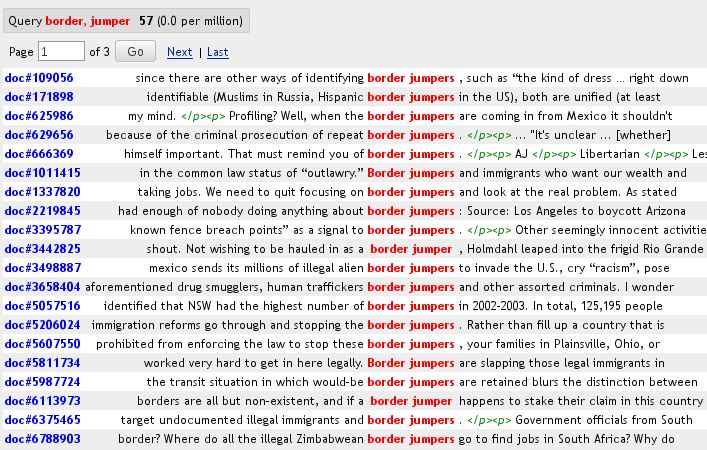
\includegraphics[width=.9\textwidth]{./figures/4-4.png}
\caption{Concordance lines, \textit{border jumpers}, GkWaC, in SketchEngine} \label{fig:2:5}
\end{figure}

\ea \label{ex:2:22}
\begin{xlist}
\exi{}[\textbf{[EN]}]{I mean, Christ, Lincoln \emph{freed the slaves}, what, like hundred and thirty years ago. \emph{How long does it take to get your act together}?}
\exi{}[\textbf{[EL]}]{Ο Λίνκολν \emph{απελευθέρωσε τους σκλάβους} πριν 130 χρόνια. \emph{Πόσον καιρό χρειάζεσαι για να γίνεις άνθρωπος;}}
\exi{}[\textbf{[Back translation]}]{Lincoln \emph{freed the slaves} a hundred and thirty years ago. How long does it take to become a human?}
\end{xlist}
\z

During a family dinner, Derek argues with his professor (who apparently has an affair with his mother) about riots in the black neighbourhoods. Example \REF{ex:2:22} comes to reinforce his argument that the sheer number of jailed black people proves their racial commitment to crime. The idiom used in this example, \textit{get one's act together}, has the meaning of getting organised and being on schedule. The utterance is implicitly ironic. In our study, the source segment has been noted as a negative judgement of medium strength, this being mainly due to the ironic nature of both the argument and the reference to the end of slavery. On the other hand, the Greek translation uses the idiom \textit{γίνομαι άνθρωπος} [become human] (GkWaC frequency: 1.9 per million) which has the meaning of “becoming an ethical and useful citizen”, thus implying a shift towards a stronger negative judgement about the social attitude of black people.\newline

\ea \label{ex:2:23}
\begin{xlist}
\exi{}[\textbf{[EN]}]{We'll let the \emph{niggers, kikes and spics} grab for their piece of the pie.}
\exi{}[\textbf{[ES]}]{Dejemos que \emph{negros y latinos} se lleven su parte.}
\exi{}[\textbf{[Back translation]}]{Let the \emph{blacks} and the \emph{Latinos} get their part.}
\end{xlist}
\z

The leader of the skinhead gang, a middle-aged male, tries to convince Derek that their organisation is going to stop being a small gang and will now grow into something very serious and powerful all over the country. He explains how he plans to act in order to achieve it.

In example \REF{ex:2:23} above, we mark the use of three racial slurs, \textit{nigger} (enTenTen12 frequency: 0.9 per million) as highly negative appreciations towards Jews, Latinos, and black people respectively. In the Spanish \textsc{tt}, the racial slurs of the original are shifted towards neutralisation (\textit{negros} and \textit{latinos}), while the reference to Jews (\textit{kikes}) is eliminated. In all, the negative appreciations that are inherent in racial slurs are eliminated. Although in Spanish there is a lexeme, \textit{negrata}, which has the same derogatory connotation as \textit{nigger}, translating \textit{nigger} as \textit{negro} is a recurrent practice in our corpus. However, \textit{negrata} is a term with a very low frequency (only 97 tokens in esTenTen11), while \textit{nigger} appears with a frequency of 0.9 per million in enTenTen12. This observation could be indicative of the reasons that made Spanish subtitlers opt for the neutral term, avoiding the use of an uncommon term. On the other hand, \textit{spic}, a term that could have been translated as \textit{sudaca} (a Spanish racial slur with presumably similar connotations with 431 tokens in esTenTen11) is also avoided. In both cases, the translator opts for neutralising the rendition of the original utterance.

\ea \label{ex:2:24}
\begin{xlist}
\exi{}[\textbf{[EN]}]{Name your price, \emph{cracker}.}
\exi{}[\textbf{[ES]}]{Di tu precio, \emph{blanco}.}
\exi{}[\textbf{[Back translation]}]{Name your price, white guy.}
\exi{}[\textbf{[EL]}]{Πες το ποσόν, \emph{βλάχο}.}
\exi{}[\textbf{[Back translation]}]{Name your price, country bumpkin.}
\end{xlist}
\z

During a basketball game in the neighbourhood court, members of the skinhead gang start to quarrel with members of a “black gang”. Derek has a bet; he proposes a “whites against blacks” game. The answer in \REF{ex:2:24} comes from one of the opponents, indicating that they accept the bet.
In example \REF{ex:2:24} above, the disparaging term \textit{cracker} (showing negative appreciation, i.e. for a poor white person, usually from the South) is translated as \textit{blanco} [white] in Spanish, but as \textit{βλάχο} [country bumpkin] in Greek. In this case, the Spanish subtitler succeeds in maintaining the racial nuance of the term, although the strength of the negative appreciation is diminished, while the Greek subtitler eliminates the racial reference and only transfers the aggressive tone of the dialogue. 

\ea \label{ex:2:25}
\begin{xlist}
\exi{}[\textbf{[EN]}]{- Do you speak English? - I am speaking English, you stupid cow!}
\exi{}[\textbf{[EL]}]{- Θα μιλήσετε Αγγλικά; - Μιλάω Αγγλικά!}
\exi{}[\textbf{[Back translation]}]{- Are you going to speak English? - I speak English!}
\end{xlist}
\z

In example \REF{ex:2:25} above, an Asian woman enters a hospital screaming the name of her husband. The intuitive reaction of the nurse is to ask her if she speaks English, a reaction reflecting the stereotype that immigrants do not speak the language of the host country. Thus, we mark this instance as a low strength negative appreciation, yet expressed in a polite manner. The Greek subtitler opts for a more aggressive-impolite way in rendering this question, \textit{θα μιλήσετε Αγγλικά} [Are you going to speak English?] strengthening the negative valence of the utterance. There are many similar examples in our corpus, pointing to the linguistic identity as a marker of difference. \citet[111]{Sella2001} argues that language is involved in matters of political and social texture, by functioning as the defining element of the nature of multiple human groupings, either positively by delineating “Us”, or negatively, by excluding allophones from the said group: in this case, the interlocutors are self-determined contrastingly, both within and outside a linguistic group (the “Others”).

\ea \label{ex:2:26}
\begin{xlist}
\exi{}[\textbf{[EN]}]{Stupid \emph{wetback}}
\exi{}[\textbf{[ES]}]{Estúpida \emph{sin papeles}}
\exi{}[\textbf{[Back translation]}]{Stupid undocumented immigrant}
\end{xlist}
\z

In \REF{ex:2:26}, an Asian and a Latin American woman are involved in a car crash. While they quarrel, the first one calls the other a \textit{wetback}. The term is highly disparaging and refers to illegal Latin Americans (especially Mexicans) as a descriptor of the way Mexicans enter the US, crossing the Rio Grande. Therefore, it has been marked as a negative judgement utterance. Although the term is decades-old and has been used even in the title of a deportation programme of the US in 1954 (the so-called “Operation Wetback”, see \citealt{Hernandez2006}), today it is used in a highly derogatory manner as a racial slur. As shown in \figref{fig:2:6}, the most significant collocations of wetback (sorted by Mutual-Information, in a query window of {-10 to +10} tokens) are other racial slurs, especially in their context of usage (e.g. \textit{mojado}, \textit{beaners}, \textit{spics}, \textit{kike}, \textit{nigger}, \textit{Chink}, \textit{greaser}, \textit{lowlife}, etc.).

\begin{figure}
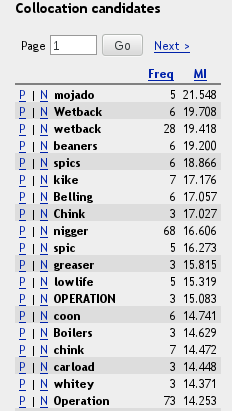
\includegraphics[width=.3\textwidth]{./figures/4-5.png}
\caption{Collocates of \emph{wetback} in enTenTen12, sorted by Mutual Information (MI) in SketchEngine} \label{fig:2:6}
\end{figure}

On the other hand, the Spanish translation uses \textit{sin papeles} [undocumented immigrants]. This is a rather neutral term to refer to illegal immigrants. In esTenTen11, the most significant collocates of \textit{sin papeles} (see \figref{fig:2:7}) are emotionally neutral (\textit{inmigrante} [immigrants], \textit{empadronar}/\textit{empadronamiento} [inclusion in the town registry], \textit{redadas} [raids], \textit{patera}/\textit{pateras} [dinghy]) and an analysis of the concordances shows that the term is used also in texts, in support of the human rights of immigrants.

\begin{figure}
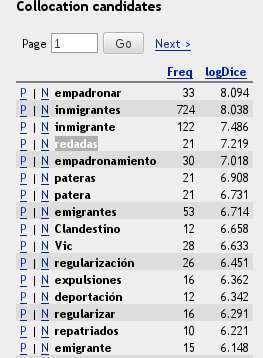
\includegraphics[width=.4\textwidth]{./figures/4-6.png}
\caption{Collocates of \emph{sin papeles} in esTenTen11, sorted by logDice in SketchEngine} \label{fig:2:7}
\end{figure}

In other words, the racist tone of the insult, even though it is still present in the Spanish text, is reduced in the interpersonal component of the utterance.

\ea \label{ex:2:27}
\begin{xlist}
\exi{}[\textbf{[EN]}]{- You wanna buy these Chinamen? - Don't be ignorant. They're Thai or Cambodian. Entirely different kind of \emph{chinks}.}
\exi{}[\textbf{[ES]}]{- ¿Vas a comprar esos chinos? -No seas ignorante. Serán tailandeses o camboyanos. Son unos \emph{amarillos} distintos.}
\exi{}[\textbf{[Back translation]}]{Should be Thai or Cambodian. They are different yellow people.}
\end{xlist}
\z

Once again, a character of \textit{Crash} uses a racial slur to refer to a group of Asians. He, quite ironically, has just decided to set them free instead of accepting money to “sell” them with the truck he robbed and proved to have been used for human trafficking. This is a negative appreciation texteme. Once again, \textit{chink} (queried in SketchEngine as a noun) was found to collocate with other racial slurs in our reference corpus. However, a similar query for \textit{amarillo} [yellow] does not yield any results, since as a noun it refers also to the colour, and in the tool used, semantic disambiguation is not possible. However, the use of a colour to designate a race does not necessarily indicate a racist stance, given that the utterance is not directed at Asians. This explanation is consistent with the definition of \textit{amarillo}, taken from the online version of the \textit{Diccionario de la Real Academia Española} \textit{(DRAE)}, which is not marked as derogatory, but as simply referring to the Asian race.\footnote{“Dicho de un individuo o de la raza a que pertenece: De piel amarillenta y ojos oblicuos. Apl. a pers., u.t.c.s.” \url{http://goo.gl/oelvVZ}.}


\subsection{Summary of findings} \label{sec:2:5:2}
Each language/culture produces and stabilises forms of expressing (racist) meanings that are unknown or at least asymmetrically\footnote{For a discussion on cultural asymmetry in translation, a concept coined in TS by \citet{EvenZohar2005}, see e.g. \citet{Klaudy2012}.} represented in other languages and cultures. Racial slurs are a clear example of this and constitute crucial points for the translator, who often mitigates or omits them. Even though the mitigation of racial slurs is the general tendency in our corpus, there are also cases of over-toning of racist attitudes, e.g. in examples \REF{ex:2:22} and \REF{ex:2:25}; in both these examples, the (racist-oriented) interpersonal meaning is intensified in the TL, though both target utterances lack marked epithets (slurs). Such instances should be explored further. This article has discussed different types of register shifts, without attempting to provide a systematic analysis (for instance, we did not consider the many instances of racist discourse which did not undergo significant register shift in translation). Such a systematic analysis, which shall be pursued in further research, will hopefully provide a more “sustainable” picture of how racist discourse is handled in translation.

\section{Conclusions} \label{sec:2:6}

This paper has presented a research, based on the PhD thesis of the first author, aimed at investigating the translation of racist discourse in Anglophone films subtitled in Greek and Spanish.

To this end, we have developed a linguistic annotation model in order to systematically categorise racism-related utterances in original films and in their subtitled versions. Instances of stereotyped views, prejudices, racist attitudes and emotions triggered by racism were coded using an annotation scheme based on Appraisal Theory.

The reference corpora used for the analysis were extremely useful, though with some limitations. Firstly, they were neither corpora of spoken discourse nor balanced corpora. Secondly, some of the terms looked up have very low frequencies and therefore do not allow a safe description. Thirdly, it was not possible to find reliable evidence for ambiguous terms such as \textit{amarillo} or \textit{sin papeles}. In many cases the meaning of a racist expression could be interpreted only by analysing its context in the film.

Our analysis of register shifts in translation, based on a Systemic Functional Linguistic approach, is promising for the descriptive study of the socio-culturally marked discourse of racism and aims to serve as an explanatory basis for addressing broader questions:

\begin{itemize}
\item Is it possible, and if so how, to refine the definitions of heterophobia that have formed part of our initial motivation in functional linguistic terms?
\item Which is the relation between cinema and socio-linguistic reality in the perception of xenophobia?
\item What are the implications of such an analysis, in relation to the comprehension of racist discourse and its root causes in the modern Greek and European linguistic and cultural reality?
\end{itemize}

Last but not least, our findings so far point to the assumption that such an approach could, indeed, be linked systematically to the critical study of the role of translation in the diachronic development of the sociolinguistic dimension of racism.

\printbibliography[heading=subbibliography,notkeyword=this]

\end{document}